\chapter{Gerência de Entrada/Saída (E/S)}

Apesar das muitas maneiras possíveis de se realizar E/S, o UNIX resolveu integrar os dispositivos no sistema de arquivos, sendo chamados de arquivos especiais. Cada dispositivo é associado a um caminho, geralmente no diretório /dev. Como exemplos temos /dev/hda como o primeiro disco rígido, /dev/lp como impressora, /dev/tty como um terminal, e /dev/sda como o primeiro dispositivo sata.

Os arquivos especiais são acessados da mesma maneira que os demais arquivos. As chamadas do sistema \emph{read} e \emph{write} são suficientes para acessa-los. Programas podem abrir, ler e escrever em arquivos especiais da mesma forma que em arquivos comuns. O comando \emph{cp}, por exemplo, não tem conhecimento que o destino para qual ele está copiando o conteúdo pode ser impressora.

Arquivos especiais são divididos em duas categorias, bloco e caractere. Um arquivo de bloco consiste de seqüências de blocos enumerados, cuja principal característica é que cada bloco pode ser acessado e endereçado individualmente. Como exemplo, podemos ler diretamente o bloco 124 sem passar pelos blocos 0 a 123. Geralmente os arquivos especiais de blocos são associados aos discos.

Normalmente, os arquivos de caracteres são empregados em dispositivos em que a entrada e a saída são feitas como fluxo de caracteres. Como exemplo, dispositivos como teclado, impressora, redes, mouses, plotters, ou seja, dispositivos que recebem e enviam dados de forma serial.

Associado ao arquivo especial, existe um driver do dispositivo que trata o dispositivo correspondente. Cada driver possui um número de dispositivo principal, que serve para identificá-lo. Se o driver suportar vários dispositivos, digamos, dois discos ao mesmo tempo, cada driver terá um número de dispositivo secundário que o identificará.

Um driver simples pode tratar também dois dispositivos relacionados, como exemplo um terminal, onde o arquivo especial /dev/tty está associado tanto ao teclado quanto a tela de vídeo, os quais são muitas vezes interpretados como um único dispositivo.

A maioria dos arquivos especiais de caracteres não pode ser acessada aleatoriamente. Esses arquivos especiais muitas vezes precisam ser controlados de uma maneira proibida aos arquivos de bloco. Uma chamada do sistema especial reservada pelo Unix configura um dispositivo de acordo com o gosto ou exigência do usuário. Essa chamada não é permitida a arquivos de blocos comuns.

\section{Rede}

A transmissão de dados em rede é baseada em sockets, introduzida no Unix de Berkeley (BSD). Os sockets são criados e destruídos dinamicamente. Sua criação retorna um registro descritor de arquivo, para estabelecer a conexão, leitura e escrita de dados e liberação da conexão. Quando o socket é criado especifica-se que tipo de transmissão ele suporta. Os tipos mais comuns são listados a seguir:

\begin{itemize}
\item Fluxo confiável de bytes orientado à conexão;
\item Fluxo confiável de pacotes orientado à conexão;
\item Transmissão não confiável de pacotes.
\end{itemize}

No fluxo confiável de bytes orientado à conexão, dois processos, em diferentes máquinas, estabelecem entre si o equivalente a um pipe. Os bytes são escritos em uma extremidade e recebidos na outra, na mesma ordem. Ele é confiável, pois existe garantia que os bytes que partem do processo emissor cheguem no receptor e na mesma ordem de envio.

O mesmo ocorre com o fluxo confiável de pacotes orientado à conexão, só que existe a divisão dos bytes em pacotes. Se o emissor efetua cinco chamadas do sistema \emph{write}, e o receptor estiver configurado como o primeiro tipo de socket, ele espera então as cinco chamadas de 512 bytes como uma só de 2560 bytes, e todos esses bytes são retornados em uma chamada. Quatro chamadas a mais são necessárias para transmitir o restante da informação.

A transmissão de dados que utilizam a transmissão não confiável de pacotes não possui nenhum controle sobre os pacotes transmitidos. Podem ser reordenados e perdidos pela rede. Na verdade, o que importa é a rapidez na transmissão e não a confiabilidade da mesma. Esse tipo de socket é útil para aplicações de tempo real e para aqueles usuários que implementaram um esquema especializado de tratamento de erro. Dá também ao usuário o acesso aos recursos de baixo nível da rede.

Depois que os sockets foram criados nos computadores origem e destino, uma conexão pode ser estabelecida entre eles.

Um lado faz uma chamada de sistema \emph{listen} (escute) no socket local. Essa chamada cria um buffer e fica bloqueada até a chegada do dado (como um \emph{receive} bloqueante). O outro lado faz a chamada de sistema \emph{connect} (conecte) passando como parâmetros o descritor de arquivos do socket local e o endereço do socket remoto. Se o lado remoto aceita a chamada, o sistema estabelece uma conexão entre os sockets.

Após o estabelecimento da conexão, o funcionamento é parecido com um pipe. Um processo pode ler e escrever nessa conexão usando o descritor de arquivos do socket local. Quando ela não é mais necessária, pode ser fechada com uma chamada de sistema \emph{close}.

\section{Chamadas do Sistema para Entrada / Saída}

Como já vimos, cada dispositivo de E/S no sistema Unix está associado a um arquivo especial. A maioria das E/S podem ser feitas acessando o arquivo correto, dispensando o uso de chamadas do sistema. Porém algumas vezes pode ser necessário que o dispositivo faça algo em particular. Podemos ver algumas chamadas do sistema na \ref{tab:chamadas_sistema}.

\begin{table}
\caption{Chamadas do Sistema UNIX de E/S}
\label{tab:chamadas_sistema}
$s = cfsetospeed(\&termios, speed)
Ajusta a taxa de transferência de saída.
s = cfsetispeed(\&termios, speed)
Ajusta a taxa de transferência de entrada.
speed = cfgetospeed(\&termios)
Obtém a taxa de transferência de saída.
speed = cfgetispeed(\&termios)
Obtém a taxa de transferência de entrada.
s = tcsetattr(fd, opt, \&termios)
Ajusta os atributos.
s = tcgetattr(fd, \&termios)
Obtém os atributos.$
\end{table}

A estrutura \emph{termios} representa a configuração de um dispositivo, \emph{speed} é uma enumeração com as possíveis taxas de transferência, \emph{fd} é um descritor de arquivo aberto, e \emph{s} é um inteiro que indica se ocorreu algum erro.

As duas primeiras funções ajustam na estrutura passada a taxa de transferência, mas ela não tem efeito imediato. Para que a taxa seja atualizada, é preciso usar a função \emph{tcsetattr}, que recebe \emph{opt}, o qual indica e momento em que os novos atributos passarão a ter efeito. Essa função na verdade serve para atualizar qualquer atributo do dispositivo.

\subsection{ioctl}

A ioctl é uma chamada do sistema anterior ao padrão POSIX que executa inúmeras ações específicas dos dispositivos, nos seus arquivos especiais. Com o tempo, ela tornou-se confusa e o POSIX distribuiu suas funções em chamadas distintas.

Existem outras chamadas a funções de E/S e a ioctl ainda existe na maioria dos sistemas Unix.

\section{Implementação da Entrada / Saída}

A implementação da E/S no Unix é feita por um conjunto de drivers de dispositivo, sendo um, normalmente, para cada tipo de dispositivo.

Quando um arquivo especial é acessado, o sistema de arquivos determina os números do dispositivo principal e secundário pertencentes a ele e que tipo de arquivo especial ele é. O número do dispositivo principal indexa ou a tabela interna \emph{bdevsw}, para arquivos de blocos, ou a tabela interna \emph{cdevsw}, para arquivos de caracteres.

Essas duas estruturas possuem ponteiros para os procedimentos das chamadas do sistema de abertura, leitura e escrita no dispositivo.
$
\begin{table}
\caption{TODO}
\label{tab:}
TODO: referencia.
\end{table}$

O número do dispositivo secundário é passado como parâmetros. Quando um novo dispositivo é inserido no sistema Unix, é incluído uma nova entrada em uma dessas tabelas e são fornecidos os procedimentos responsáveis pelo tratamento das operações deste dispositivo.

Na tabela \emph{cdevsw} cada linha contém ponteiros para as funções suportadas por um driver. Quando uma operação é executada em um arquivo especial de caractere, o sistema indexa a tabela cdevsw para selecionar a linha correspondente ao dispositivo e chama a coluna correspondente à função requisitada.

Um driver de dispositivo para sistemas Unix tem a metade superior fazendo a interface com o restante do Unix no contexto de quem requisita (chama) o dispositivo. E a metade inferior interagindo com o dispositivo e executando no contexto do kernel do sistema. Por questões de segurança, os drivers podem chamar apenas algumas funções do kernel, e o conjunto delas está definida em um documento chamado Interface Driver-Kernel.

O sistema de gerência de E/S é divido em dois grandes componentes: o tratamento de arquivos especiais de bloco e o tratamento de arquivos especiais de caractere.

O objetivo do tratador de arquivos de bloco \ref{fig:tratadores} é minimizar o número de transferências que devem ser feitas envolvendo o disco. Para isso possui uma cache de blocos (buffer cache) entre os drivers do disco e o sistema de arquivos. Essa cache é uma tabela no kernel com a finalidade de armazenar os blocos mais recentemente usados. Quando um bloco é requisitado, uma verificação é feita para confirmar se ele já não está no buffer cache. Se ele está lá, o acesso ao disco é poupado e o dado é recuperado da cache, senão, é lido do disco e colocado na cache de blocos, e de lá copiado para quem o chamou.

\begin{figure}
	\caption{Tratador de arquivos de bloco e caractere}
	\label{fig:tratadores}
	\centerline{
		\scalebox{0,8}{
			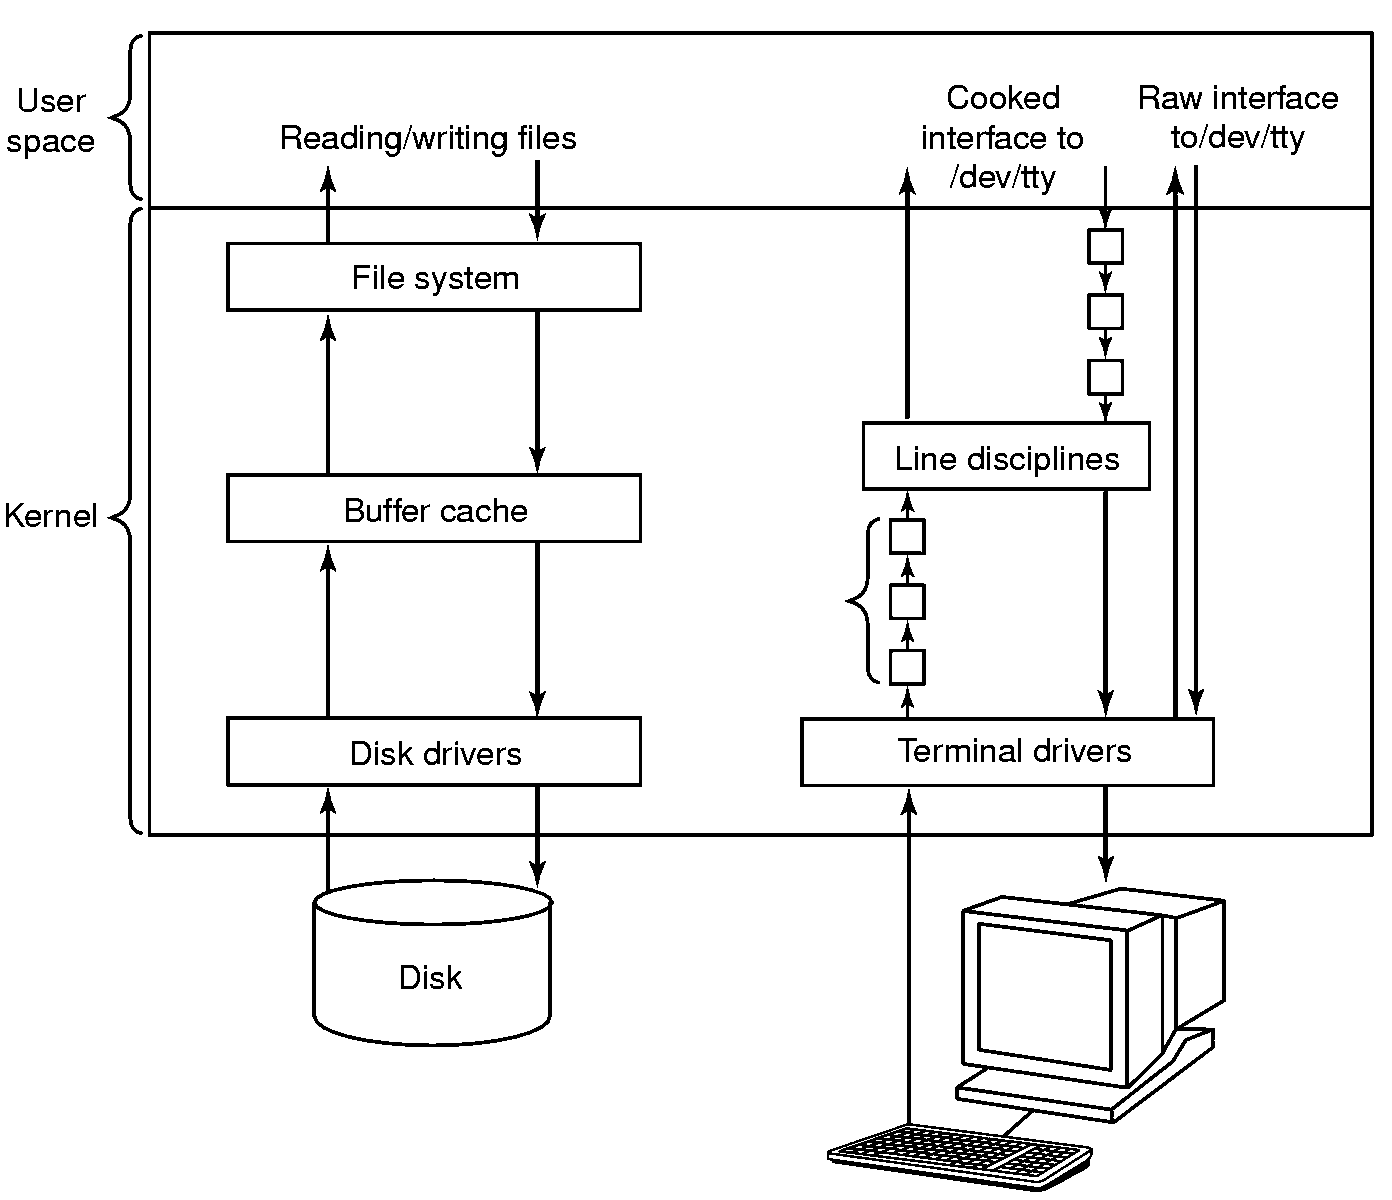
\includegraphics{imgs/unixIOsystem.png}
		}
	}
\end{figure}

A cache é de tamanho fixo e necessita de um algoritmo para gerenciá-la. Em geral, seus blocos encontram-se em uma lista encadeada, onde os acessos são movidos para a cabeça da lista. Quando o algoritmo de gerenciamento da cache remove um bloco, retira-o final da cadeia, pois é aquele que foi menos recentemente usado.

A escrita, da mesma forma, necessita que os blocos sejam copiados para a cache primeiramente e depois para o disco. Quando ela é preenchida e precisa ser liberada, os blocos vão para o disco. A cada 30 segundos os blocos modificados no dispositivo são gravados, afim de quem não esperem para sempre no buffer cache.

\subsection{Instalação de novos drivers}

Nos sistemas Unix originais, onde os drivers dos dispositivos eram linkados estaticamente no núcleo, uma atualização de hardware necessitava de uma nova linkagem do kernel. Com o advento dos computadores pessoais e seus inúmeros dispositivos de E/S disponíveis, a maioria dos usuários Unix/Linux sente dificuldade para incluir seus drivers, atualizar as tabelas, re-linkar o kernel e reinicializar o sistema.

O sistema operacional Linux resolveu essa dificuldade com os módulos carregáveis, que são blocos de códigos vinculados ao núcleo, em tempo de execução. Podem ser drivers que se utilizam de arquivos especiais, ou módulos mais complexos, como sistemas de arquivos, protocolos de rede, etc.

Quando um modulo é carregado, várias coisas precisam ser feitas. O módulo deve ser relocado durante o carregamento. Depois o sistema deve verificar se os recursos necessários estão disponíveis. Então, os vetores de interrupção são atualizados. Em seguida, a tabela \emph{bdevsw} ou \emph{cdevsw} é atualizada. Finalmente o driver é executado para fazer qualquer inicialização de que necessite.

\section{Streams}

Arquivos especiais de caracteres não utilizam o buffer cache e sim, usam o fluxo de caracteres. Nas primeiras versões do Unix, cada drive do dispositivo de caracteres devia fazer tudo para que seu dispositivo funcionasse, mas com o passar do tempo, a maioria dos drivers continha código que executava as mesmas funcionalidades, como tratamento de buffer, controle de fluxos e protocolos de rede. Duas soluções foram então criadas para contornar esse problema.

C-lists, a solução BSD, são blocos de até 64 caracteres com um contador e um ponteiro para o próximo bloco. Caracteres que chegam dos dispositivos vão sendo colocados em uma cadeia desses blocos. Quando existe leitura por um processo no arquivo correspondente ao dispositivo, /dev/tty, esses caracteres passam por uma parte do código do kernel denominada de tratador de linhas (line discipline) que age como filtro produzindo um fluxo de caracteres preparado (cooked character stream), onde processamentos especiais foram aplicados. Esse fluxo preparado é então passado para processo.

A saída é feita de modo semelhante, só que inserindo caracteres especiais ao invés de retirá-los.

Na solução system V, planejada por Dennis Ritchie, os fluxos ou streams são de aplicação mais geral. Sua idéia principal é facilitar a comunicação de um processo do usuário com o driver do dispositivo, bem como a inserção de módulos durante a execução, como pode ser visto em \ref{fig:system_V}.

Os fluxos possuem um cabeçalho no topo e uma conexão com um driver em sua base. Quando um processo do usuário escreve em um fluxo, o código presente no cabeçalho interpreta a chamada do sistema e empacota os dados em buffers do fluxo, que vão passando de módulo a módulo, em filas de leitura e escrita distintas. Os módulos executam algum tipo de transformação pré-definida e podem ser também módulos de multiplexação, onde capturam um fluxo e os dividem em vários fluxos ou vice-versa.

\begin{figure}
	\caption{Solução system V}
	\label{fig:system_V}
	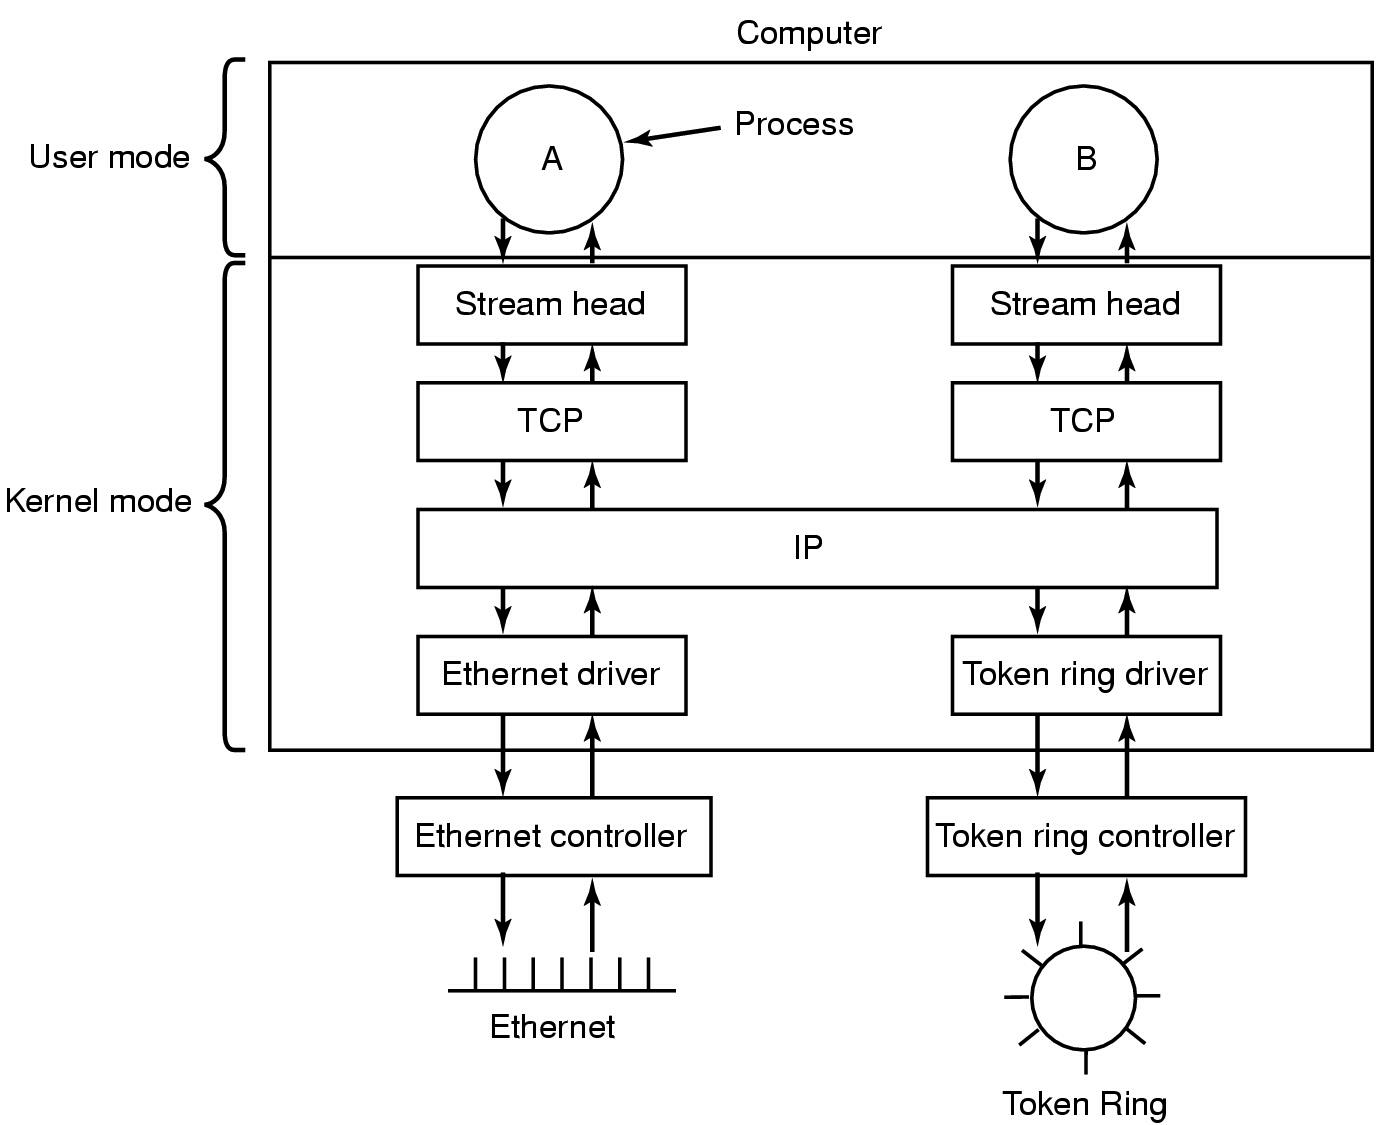
\includegraphics{imgs/systemVstreams.png}
\end{figure}
